\documentclass[11pt]{article}
\usepackage[margin=1in]{geometry}
\usepackage{booktabs,graphicx,hyperref,amsmath,url,xcolor}
\usepackage[utf8]{inputenc}
\usepackage[T1]{fontenc}
\hypersetup{colorlinks=true,linkcolor=blue!60!black,citecolor=blue!60!black,urlcolor=blue!60!black}

\title{handnet: Neural Networks with Hand-Written Weights}
\author{Birger Mo\"ell\\ Uppsala University, KTH, AI Sweden \and Claude\\ Anthropic (wrote the weights and code, in conversation with the first author)}
\date{Draft, November 2026}

\begin{document}
\maketitle

\begin{abstract}
% TODO(paper thread): finalise once the second and third networks and the ablations exist.
We study neural networks whose weights are \emph{designed} rather than learned. The
architecture is standard (embeddings, convolutions, ReLU recurrences, multilayer
perceptrons), the tensors are allocated at a fixed parameter budget, and every non-zero
weight is placed by reasoning about the task; the vast majority of the budget stays zero.
We describe a small toolbox of constructions (pattern kernels, first-of-run counting,
run-length counters as a ReLU recurrence with a closed form, capped detectors from ReLU
pairs, $\min$ gates, count-then-threshold) that lets ordinary task knowledge be written
directly as weights, and we report experiments on four networks across three tasks. A
multilingual text-quality network of 100{,}331 parameters (627 non-zero) separates kept
from removed FineWeb-2 documents with a mean AUC of 0.907 over 33 languages and eleven
scripts (0.82--0.98) without having seen a document, beating single-statistic baselines
in all but one language. An SST-2 sentiment network written blind reaches 78.6\,\%, and
two MNIST designs reach 79.4\,\% (weights that are ASCII drawings, written blind with
bounded revisions) and 83.3\,\% (hand-drawn stroke kernels, a recurrent hole finder,
$5\times5$ sketches and named evidence units; above a trained nearest-class-mean
classifier at 81.6\,\%). Label-matched trained baselines show where designed weights
win and where a few hundred labels beat the best drawing. We discuss where the approach stops (knowledge that
cannot be articulated in the input features, such as morphology or whether a loop
closes), and how designed networks relate to trained ones as initialisations, baselines
and specifications. Code, results and an in-browser demo are at
\url{https://birgermoell.github.io/handnet/}.
\end{abstract}

\section{Introduction}
% TODO(paper thread): motivation. Points to make:
% - A trained 100k model uses every weight a little; a designed one uses a few hundred a lot.
% - Explanation is the network, not an attribution method.
% - Data-free: no leakage, no corpus bias, identical behaviour across languages/scripts.
% - Starting observation (Lauritzen, 2026): an LLM asked to hand-write weights for a
%   100k-param citation classifier used 3.8k non-zero weights and beat the trained version
%   (97.8% vs 94.6% at 8k labels). We ask how far this carries and how to do it by hand.

\section{Related work}
Hand-designed features with a learned classifier are the pre-deep-learning norm; here
the classifier is hand-designed too. The closest precedents are the rule-based quality
filters of large pretraining corpora---C4 \cite{raffel2020t5}, Gopher \cite{rae2021gopher},
FineWeb and FineWeb-2 \cite{penedo2024fineweb,penedo2025fineweb2}---whose rules (fraction
of letters, mean word length, lines ending in punctuation, repetition ratios) our text
network reimplements as network units with a shared scoring scheme and script gating.
The starting observation for this work is a report that a language model asked to
hand-write the weights of a 100k-parameter citation classifier used 3.8k non-zero
weights and beat the trained version \cite{lauritzen2026fable}. Network ``circuits'' with
interpretable weights are the object of mechanistic interpretability \cite{olah2020zoom};
we build circuits forward instead of reverse-engineering them. Hand-set recurrent
counters resemble the constructions used to show what RNNs can compute in principle
\cite{weiss2018counter}, and our hole finder is a cellular-automaton flood fill written
as a ReLU recurrence. MNIST \cite{lecun1998mnist} needs no introduction;
template-matching and nearest-prototype classifiers are its oldest baselines, and our
sketch units are nearest-prototype with prototypes drawn by hand. Sparse networks are
usually obtained by pruning a trained one \cite{frankle2019lottery}; ours are sparse by
construction, with the sparsity pattern carrying the design.

\section{Method}
% Method section. Owner: text-quality thread (claude-13); additive edits welcome.
\subsection{Setting}
A hand-written network is an ordinary feed-forward or recurrent network
$f_\theta$ whose parameter tensors are allocated at a fixed budget and
initialised to zero, after which individual entries are set by the author.
We require that (i) every layer is a standard operation (affine map, ReLU,
convolution, ReLU recurrence, mean/max pooling), so that $\theta$ loads into
any deep-learning framework unchanged, and (ii) every non-zero entry carries a
comment stating why it has its value. We report two numbers for each network:
the allocated parameter count $|\theta|$ and the number of non-zero entries
$\|\theta\|_0$.

\subsection{Input representation}
The weights are only as readable as the features they read. We therefore use
inputs whose meaning is fixed a priori and make the first embedding the
identity. For text, each character is mapped to a binary attribute vector
(Unicode general category, case, script block, punctuation class, combining
mark, a same-as-previous-character bit, and a few task-specific markers such
as the lead and tail bytes of UTF-8 mojibake). No vocabulary is involved, so
one set of weights applies to every language and script.

\subsection{Constructions}
Six constructions account for every non-zero weight in the networks reported
here.

\paragraph{Pattern kernels.} A convolution channel with weight $1$ on each
required (offset, attribute) pair and bias $-(n-1)$ fires under ReLU only when
all $n$ attributes are present: $\mathrm{relu}(\text{terminal}_{t-2} +
\text{space}_{t-1} + \text{upper}_t - 2)$ detects a sentence start in cased
scripts. A large negative weight on an attribute implements exclusion.

\paragraph{First-of-run counting.} $\mathrm{relu}(x_t - \text{same\_prev}_t)$
is $1$ only at the first character of a run of $x$, so that a separator line
of eighty dashes contributes one count rather than eighty.

\paragraph{Run-length counters.} A ReLU recurrence
$h_t=\mathrm{relu}(h_{t-1}+u_t)$ with unit self-weight and input
$u_t = \text{inc}_t - B\cdot\text{reset}_t$ ($B$ large) counts increments since
the last reset: characters since the last space (word length), since the last
sentence end (sentence length), words since the last sentence end. Because the
self-weight is exactly $1$, the recurrence has the closed form
$h_t = S_t - \min(0,\min_{k\le t} S_k)$ with $S$ the cumulative sum of $u$
(the Lindley recursion), so inference is vectorised; the step-by-step
recurrence is used for the PyTorch export and the two are tested to agree.

\paragraph{Capped detectors.} A penalty that rises from $0$ at threshold $a$
to its full value at $b$ and saturates is $\min(\mathrm{relu}(x),1) =
\mathrm{relu}(x) - \mathrm{relu}(x-1)$ with $x$ an affine function of the
pooled features scaled so that $x=1$ is ``fully bad''. The next layer multiplies
the pair by a point budget. Every penalty and reward term is one such unit, and
the sum of the named terms is the output; this is what makes
\texttt{explain()} exact rather than approximate.

\paragraph{Gates.} A detector that is meaningless for some input mode (word
length when the script has no spaces; capitalisation when the script has no
case) receives a weight of $-100$ on the rate of that mode. A soft gate
$\min(g,p)$, used to switch rate-based penalties on only once the document is
long enough for rates to be meaningful, costs one extra layer:
$p - \mathrm{relu}(p-g)$.

\paragraph{Count-then-threshold.} ``More than one script present'' is one
capped unit per script, summed with bias $-1$ and passed through ReLU; the
output is the number of extra scripts, itself capped.

\subsection{Budgets and naming}
The output is a base value plus named reward terms minus named penalty terms,
grouped into sub-scores and clipped to the target range by a final
$\mathrm{relu}(z)-\mathrm{relu}(z-100)$. Budgets are chosen in output units:
in the text-quality network a markup rate above 10\% can cost at most 20 of 100
points, mojibake at most 35, and the rewards for the shape of running prose sum
to 28, so that clean prose reaches 100 and a table reaches 0.

\subsection{Development protocol}
We develop against three sources in order: (1) hand-written samples across
scripts and junk types, each a test case with a stated reason; (2) a labelled
external set the network has never seen; (3) the worst mistakes in both
directions on (2), fixed at the level of the mechanism rather than the sample.
Every fix is recorded as a comment in the code and a line in
Section~\ref{sec:tq-devlog}. The network never sees a training signal; the
author does.

% Method: the comparison protocol used for sentiment and MNIST. Owner: claude (sentiment/MNIST thread).
\subsection{Protocol for comparing designed and trained weights}
\label{sec:protocol}

The sentiment and MNIST experiments follow a protocol that turns ``the designed
network works'' into ``the designed network is worth $N$ labels'':
(1)~freeze a differentiable architecture, building $\min$ and clipping from ReLUs so
that a trained model of the same shape is a meaningful baseline;
(2)~name every unit;
(3)~write all non-zero weights \emph{blind}, before any labelled example from the
benchmark is seen (general domain knowledge is allowed, the data is not);
(4)~evaluate once on the sealed test set and print only aggregates;
(5)~allow a bounded number of \emph{revisions}, each of which inspects a development
sample, states a hypothesis about language or shape, changes weights and is reported
as its own row with the number of labelled examples it saw, the earlier file being
kept so the row can be regenerated;
(6)~train the same architecture on $2^k$ labels for a range of $k$ and plot.
The author---here a language model, Claude Fable 5.1, in a chat session---may not
call any optimiser, may not grid-search over labelled data, and may not import
pre-trained resources. Fixed operations are allowed when parameter-free or hand-set
(a Gaussian blur, $\ell_2$ normalisation, max-pooling over offsets).


\section{Experiments}
% Experiments: multilingual text-quality network. Owner: claude-13.
\subsection{A 100k-parameter multilingual text-quality network}
\label{sec:text-quality}

\paragraph{Task.} Score a document in $[0,100]$ for usability as text in the
pretraining-filter sense: clean running prose versus markup, tables, logs,
mojibake, repetition, shouting, navigation lists, keyword lists, fragments and
mixed scripts. The score must be defined for every language and script with
one set of weights.

\paragraph{Architecture.} Characters $\to$ 40 binary Unicode attributes $\to$
identity embedding ($40\times40$) $\to$ width-5 convolution with 48 channels
(18 pass-through rates, 17 pattern detectors, 13 script rates) $\to$ a 16-unit
ReLU recurrence of run-length counters $\to$ pooling (channel means, counter
maxima and means, log length, bias; 82 features) $\to$ an MLP
$82\to512\to86\to16\to2\to1$. Layer~1 holds 70 capped detectors, 10
script-presence units and 2 length gates; layer~2 the named sub-scores, gates,
reward and mixed-script count; layer~3 the $\min(\text{gate},\text{penalty})$
terms; layer~4 the base-plus-terms score and its clip. In total
$|\theta|=100{,}331$ and $\|\theta\|_0=627$.

\paragraph{Script handling.} Word-based detectors are gated off by the rate of
Han, Kana and Thai-family characters; case-based detectors by Arabic, Indic,
Hangul and Georgian (Unicode classes Mkhedruli as lowercase; it is written
caseless). Sentence starts have a cased kernel (\texttt{. A}) and a caseless
kernel (an ideographic full stop U+3002 directly followed by a Han character, or a full stop, space and caseless letter as in Korean). Combining marks count as letters so that
Indic and Arabic vowel signs do not depress the letter rate. Han and Kana count
as one script. A CJK character is weighted as roughly $2.5$ Latin characters
in the length terms.

\paragraph{Evaluation data.} FineWeb-2 publishes, per language, the documents
that survived its filtering pipeline and the documents its filters removed.
We take the first 300 of each from the first shard for Swedish, German,
Finnish, Turkish, Georgian, Arabic, Hindi and Japanese (Latin, Georgian,
Arabic, Devanagari and Japanese scripts) and report AUC for kept $>$ removed.
The network was never run on these documents during development
except through the error analysis in Section~\ref{sec:tq-devlog}, which used
the same sample; a held-out shard should be added before publication
(TODO).

\begin{table}[h]\centering
\begin{tabular}{lcccccccc}\toprule
 & swe & deu & fin & tur & kat & arb & hin & jpn \\\midrule
AUC & 0.928 & 0.901 & 0.941 & 0.901 & 0.949 & 0.883 & 0.857 & 0.896 \\
mean kept & 95.2 & 95.6 & 97.4 & 94.5 & 95.2 & 88.6 & 91.9 & 90.8 \\
mean removed & 68.8 & 74.1 & 64.8 & 70.5 & 58.4 & 64.4 & 71.3 & 61.3 \\
\bottomrule\end{tabular}
\caption{FineWeb-2 kept vs removed, 300 + 300 documents per language. Scoring takes about 7\,ms per document in numpy on one CPU core.}
\end{table}

\paragraph{Hand-written samples.} Encyclopaedic paragraphs in fourteen
languages (Swedish, English, German, Georgian, Finnish, Japanese, Chinese,
Arabic, Hindi, Russian, Greek, Thai, Korean, Turkish) score 85--97. HTML scores
23, UTF-8 mojibake 48, character repetition 35, shouting 37, a markdown table
0, a navigation list 36, a server log 9, a comma-separated keyword list 57, a
list of URLs 47, U+FFFD soup 32, source code 17, a paragraph mixing five
scripts 47, a 110-character string without spaces 41 and emoji spam 24.

\paragraph{Where it fails, by construction.} On synthetic grammar pairs from
the OELLM quality-gate data (a clean one-to-three-sentence snippet against the
same snippet with one inflection change, adjacent-word swap, typo, duplicated
word or deleted function word; Swedish, Norwegian, Georgian), the network is at
chance, and most pairs are exact ties: the attribute representation carries no
morphology or word order. Deleted function words are detected slightly above
chance (62--86\%) through length alone. The highest-scoring \emph{removed}
FineWeb-2 documents are fluent machine-translated hostel listings and
site boilerplate, which have the surface shape of prose. Both failure modes are
exactly the signal a trained judge provides, and the two are complementary:
the designed network is $\sim$1000$\times$ cheaper than a 0.3B judge and can run
first.

\subsection{Development log}
\label{sec:tq-devlog}
Each entry is a mistake found on external data and the mechanism that fixed it.
\begin{enumerate}
\item Hindi prose scored 61: Devanagari vowel signs are combining marks, so
  the letter rate was 45\%. Fix: combining marks count as letters in the
  letter-rate terms (zalgo detection stays separate and is gated off for
  Indic, Arabic and Thai).
\item Japanese prose lost 12 points as ``mixed scripts'': Han and Kana were two
  scripts. Fix: one presence unit reads both rates.
\item Korean and Georgian earned no sentence reward: Korean puts a space after
  the full stop before a caseless letter; Georgian is Unicode-lowercase. Fix: a
  second sentence kernel, and Mkhedruli mapped to the caseless attribute.
\item An 80-character separator line cost 56 points through four detectors
  (repetition, punctuation runs, symbol streak, giant token). Fix:
  first-of-run counting for markup, symbol and dash rates; repetition and
  punctuation-run kernels exclude separator characters; the word-length counter
  increments only on letters and digits; the symbol-streak threshold raised.
\item One all-caps headline cost the full 15 shouting points. Fix: the caps-run
  rate needs about 15\% of the text before the penalty saturates.
\item Short texts were hit by every rate-based penalty at once (a 17-character
  sentence-splitter fragment scored 3). Fix: two length gates as
  $\min(\text{gate},\text{penalty})$; composition penalties switch on between 30
  and 100 characters, structure penalties between 100 and 300.
\item The replacement character U+FFFD was classed as a symbol, not garbage.
  Fix: attribute order.
\item Chinese and Japanese lost 4--7 points for ``comma-heavy'' text (ideographic
  commas are dense). Fix: the detector is gated off for spaceless scripts.
\end{enumerate}
No entry changed the FineWeb-2 AUC by more than $\pm0.01$; the fixes removed
false positives on individual documents (e.g.\ a Georgian medical page from 66 to
96) without moving the aggregate.

\subsection{Ablation by sub-score}
Switching off one named sub-score at a time (zeroing its layer-2 unit;
\texttt{examples/text\_quality/ablate.py}) shows that on FineWeb-2 the
\emph{formatting} group---bullet-like lines, lines that break mid-sentence,
spacing errors, ellipses, symbol streaks---carries most of the separation,
which matches what FineWeb-2's own filters (Gopher repetition and quality rules,
C4 line rules) remove. The remaining groups each contribute at most
$\sim$0.01 AUC on this data but are what separates the hand-written junk
samples (HTML, mojibake, tables, logs) that FineWeb-2's sample rarely contains.

\begin{table}[h]\centering\small
\begin{tabular}{lcccccccc}\toprule
removed group & swe & deu & fin & tur & kat & arb & hin & jpn \\\midrule
none (full)  & 0.928 & 0.901 & 0.941 & 0.901 & 0.949 & 0.883 & 0.857 & 0.896 \\
noise        & 0.925 & 0.903 & 0.943 & 0.897 & 0.948 & 0.880 & 0.856 & 0.896 \\
repetition   & 0.928 & 0.901 & 0.941 & 0.899 & 0.946 & 0.873 & 0.849 & 0.893 \\
composition  & 0.925 & 0.899 & 0.942 & 0.900 & 0.948 & 0.883 & 0.857 & 0.894 \\
formatting   & 0.847 & 0.839 & 0.905 & 0.870 & 0.923 & 0.809 & 0.824 & 0.844 \\
tokens       & 0.924 & 0.902 & 0.944 & 0.901 & 0.949 & 0.889 & 0.857 & 0.896 \\
structure    & 0.928 & 0.901 & 0.940 & 0.899 & 0.946 & 0.882 & 0.851 & 0.896 \\
length       & 0.928 & 0.900 & 0.940 & 0.898 & 0.947 & 0.879 & 0.855 & 0.891 \\
\bottomrule\end{tabular}
\caption{Leave-one-group-out ablation, AUC kept vs removed.}
\end{table}

% Experiments: text quality across 33 languages, with baselines and ablation. Owner: claude (mnist/site thread, 2026-11-04). Additive to text_quality.tex.
\subsection{Text quality across 33 languages, against single-statistic baselines}
\label{sec:text-33}

Section~\ref{sec:text-quality} evaluated eight languages. Here the same protocol (first
300 kept and 300 removed documents of the first FineWeb-2 shard, AUC for kept $>$
removed) is run on 33 languages across eleven scripts (\texttt{examples/text\_quality/eval\_fineweb2.py};
Persian is not published in this layout and was skipped). As baselines, the same
documents are scored with single statistics of the kind used by rule-based filters
\cite{rae2021gopher,raffel2020t5}: $\log$ length, the fraction of characters that are
letters, the fraction of tokens containing a letter, and the Gopher-style distance of the
mean word length from 5.

\begin{figure}[t]\centering
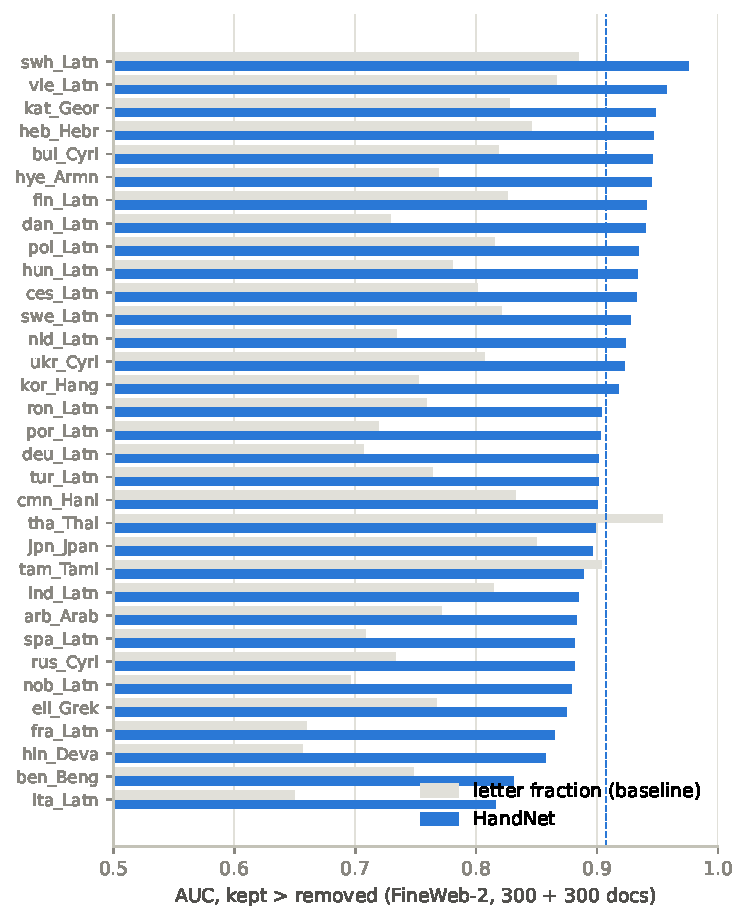
\includegraphics[width=0.62\linewidth]{figures/fineweb2_auc}
\caption{AUC(kept $>$ removed) per language, the text-quality network versus the
letter-fraction baseline. Dashed line: mean over languages (0.907).}
\label{fig:auc}
\end{figure}

\begin{table}[t]\centering\footnotesize
\caption{FineWeb-2 kept vs removed, 300 + 300 documents per language. AUC for the
text-quality network and for three single-statistic baselines; mean network score of
kept and removed documents.}
\label{tab:fineweb}
\begin{tabular}{lrrrrrr}
\toprule
language & network & length & letters & words & kept mean & removed mean \\
\midrule
swh\_Latn & 0.976 & 0.736 & 0.885 & 0.902 & 92.2 & 44.8 \\
vie\_Latn & 0.958 & 0.698 & 0.866 & 0.915 & 92.9 & 63.7 \\
kat\_Geor & 0.949 & 0.697 & 0.827 & 0.858 & 95.2 & 58.4 \\
heb\_Hebr & 0.947 & 0.643 & 0.846 & 0.886 & 93.0 & 58.6 \\
bul\_Cyrl & 0.946 & 0.668 & 0.819 & 0.873 & 96.0 & 66.9 \\
hye\_Armn & 0.945 & 0.534 & 0.769 & 0.763 & 93.5 & 57.0 \\
fin\_Latn & 0.941 & 0.696 & 0.826 & 0.861 & 97.4 & 64.8 \\
dan\_Latn & 0.940 & 0.657 & 0.729 & 0.803 & 95.3 & 66.5 \\
pol\_Latn & 0.934 & 0.643 & 0.815 & 0.818 & 95.4 & 64.5 \\
hun\_Latn & 0.933 & 0.705 & 0.780 & 0.854 & 96.3 & 64.4 \\
ces\_Latn & 0.932 & 0.675 & 0.801 & 0.852 & 95.1 & 62.3 \\
swe\_Latn & 0.928 & 0.671 & 0.821 & 0.882 & 95.2 & 68.8 \\
nld\_Latn & 0.924 & 0.638 & 0.734 & 0.846 & 94.8 & 68.8 \\
ukr\_Cyrl & 0.923 & 0.668 & 0.807 & 0.853 & 95.7 & 64.7 \\
kor\_Hang & 0.918 & 0.492 & 0.752 & 0.850 & 80.4 & 41.5 \\
ron\_Latn & 0.904 & 0.631 & 0.759 & 0.836 & 93.6 & 68.7 \\
por\_Latn & 0.903 & 0.637 & 0.720 & 0.770 & 94.0 & 67.0 \\
deu\_Latn & 0.901 & 0.628 & 0.707 & 0.849 & 95.6 & 74.1 \\
tur\_Latn & 0.901 & 0.604 & 0.764 & 0.780 & 94.5 & 70.5 \\
cmn\_Hani & 0.900 & 0.559 & 0.832 & 0.709 & 91.1 & 62.2 \\
tha\_Thai & 0.899 & 0.571 & 0.955 & 0.862 & 85.6 & 64.3 \\
jpn\_Jpan & 0.896 & 0.533 & 0.850 & 0.749 & 90.8 & 61.3 \\
tam\_Taml & 0.889 & 0.682 & 0.904 & 0.881 & 96.0 & 73.6 \\
ind\_Latn & 0.885 & 0.631 & 0.815 & 0.796 & 95.3 & 75.3 \\
arb\_Arab & 0.883 & 0.612 & 0.771 & 0.832 & 88.6 & 64.4 \\
spa\_Latn & 0.882 & 0.651 & 0.708 & 0.787 & 94.2 & 74.3 \\
rus\_Cyrl & 0.881 & 0.607 & 0.733 & 0.805 & 95.9 & 75.8 \\
nob\_Latn & 0.879 & 0.593 & 0.696 & 0.783 & 94.8 & 71.7 \\
ell\_Grek & 0.875 & 0.646 & 0.767 & 0.854 & 94.1 & 69.6 \\
fra\_Latn & 0.865 & 0.659 & 0.659 & 0.805 & 94.1 & 74.2 \\
hin\_Deva & 0.857 & 0.604 & 0.656 & 0.733 & 91.9 & 71.3 \\
ben\_Beng & 0.831 & 0.599 & 0.748 & 0.775 & 93.8 & 74.6 \\
ita\_Latn & 0.816 & 0.650 & 0.650 & 0.722 & 93.1 & 76.4 \\
\midrule
\textbf{mean (33)} & \textbf{0.907} & 0.634 & 0.781 & 0.823 & & \\
\bottomrule
\end{tabular}
\end{table}

\begin{figure}[t]\centering
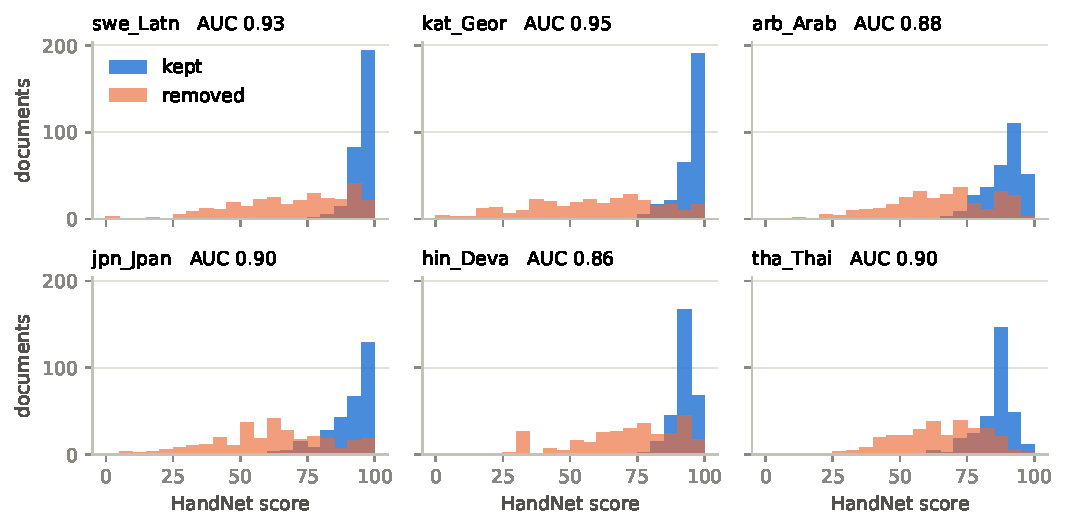
\includegraphics[width=\linewidth]{figures/fineweb2_hist}
\caption{Score distributions of kept (blue) and removed (orange) documents for six scripts.}
\label{fig:hist}
\end{figure}

Figure~\ref{fig:auc} and Table~\ref{tab:fineweb} give the results. The mean AUC is 0.907,
with every language above 0.81; Swahili (0.976), Vietnamese (0.958), Georgian (0.949),
Hebrew (0.947), Bulgarian (0.946) and Armenian (0.945) are highest, Italian (0.816),
Bengali (0.831) and Hindi (0.857) lowest. Scores of kept documents are tightly
concentrated near 95 while removed documents spread over the whole range
(Figure~\ref{fig:hist}); with a threshold of 50 essentially no kept document is rejected
in any language, and between 5\,\% (Italian) and 59\,\% (Korean) of removed documents
are.

Two observations. First, the letter fraction alone is a strong baseline (mean 0.78),
and for Thai it beats the network (0.955 vs 0.899): Thai has no sentence punctuation and
no word spaces, so the script gates switch off most of the structure detectors and little
is left. Second, FineWeb-2's own removal decisions are rule-based, so part of what is
measured is agreement between two rule systems rather than ground-truth quality; the
comparison still tells us that a 627-weight network reproduces most of a production
filtering pipeline's decisions in 33 languages.

In every language the most frequent penalties on removed documents are
\texttt{broken\_lines} (line breaks mid-sentence), \texttt{bullet\_lines} and
\texttt{fragments}, i.e.\ navigation lists and layout text, followed by
\texttt{few\_sentence\_ends} and \texttt{markup}.

\paragraph{Ablation over 33 languages.} Table~\ref{tab:ablation33} repeats the
leave-one-group-out ablation of Section~\ref{sec:text-quality} on all 33 languages, now
including the mixed-script penalty and the rewards
(\texttt{examples/text\_quality/ablate\_groups.py}). Only the \emph{formatting} group
matters much: without it the mean AUC drops from 0.907 to 0.858 and Thai from 0.90 to
0.69. The other groups are nearly redundant on this benchmark, and removing the
\emph{rewards} or the \emph{tokens} group slightly \emph{improves} the AUC. This is a
useful negative result for the design method: several detectors that are easy to
justify (shouting, digit runs, giant tokens) contribute nothing measurable to agreement
with FineWeb-2, and the reward units, which were meant to make the scale interpretable,
cost a little discrimination.

\begin{table}[t]\centering\small
\caption{Ablation over 33 languages: mean AUC with one group switched off.}
\label{tab:ablation33}
\begin{tabular}{lrrl}
\toprule
variant & mean AUC & $\Delta$ & worst language \\
\midrule
full & 0.907 & -- & 0.816 (ita\_Latn) \\
without noise & 0.905 & -0.003 & 0.810 (ita\_Latn) \\
without repetition & 0.904 & -0.003 & 0.809 (ita\_Latn) \\
without composition & 0.906 & -0.001 & 0.816 (ita\_Latn) \\
without formatting & 0.858 & -0.049 & 0.688 (tha\_Thai) \\
without tokens & 0.909 & +0.001 & 0.815 (ita\_Latn) \\
without structure & 0.906 & -0.002 & 0.820 (ita\_Latn) \\
without length & 0.905 & -0.003 & 0.806 (ita\_Latn) \\
without mixed\_scripts & 0.907 & -0.001 & 0.817 (ita\_Latn) \\
without reward & 0.913 & +0.006 & 0.830 (ita\_Latn) \\
\bottomrule
\end{tabular}
\end{table}

% Experiments: sentiment on SST-2. Owner: claude (sentiment/MNIST thread).
\subsection{A 1.5k-parameter sentiment classifier for SST-2}
\label{sec:sentiment}

\paragraph{Task.} SST-2 is the binary Stanford Sentiment Treebank \cite{socher2013}:
single movie-review sentences, lower-cased and pre-tokenised (\texttt{does n't}),
labelled positive or negative. We use the GLUE split (6{,}919 train / 872 dev / 1{,}821
test). It is hard for lexicon methods because of negation (``not a bad film at all''),
contrast (``boring at first but ultimately moving'') and intensified negatives used
as praise (``painfully funny'').

\paragraph{Architecture.} Tokens $\to$ embedding $V\times6$ $\to$ a gated recurrent
cell with state $[\,\mathrm{pos\_acc},\mathrm{neg\_acc},\mathrm{neg\_gate},
\mathrm{int\_gate}\,]$ $\to$ $\mathrm{Linear}(4\to6)$, ReLU, $\mathrm{Linear}(6\to1)$,
sigmoid. The six embedding axes are \emph{pos}, \emph{neg} (strengths 1--3),
\emph{negator}, \emph{intensifier}, \emph{contrast} and \emph{hedge}; the embedding
is therefore a typed sentiment lexicon of about 1{,}100 words. The cell is ten
scalars, each a statement about English: the negation gate decays by $0.72$ per
token (reaching about three words) and is cancelled by a following hedge (``not
\emph{just} hilarious''); a contrast word multiplies the accumulated history by
$0.35$; a word under negation is routed to the opposite accumulator at $0.65$
(pos$\to$neg) or $0.75$ (neg$\to$pos) of its strength; intensifiers multiply by
$1+\mathrm{int\_gate}$, hedges by $1-0.5\,\mathrm{hedge}$. All clipping is built from
ReLUs. The readout's six units are net sentiment, net negativity, any positivity, any
negativity, emotional mass and dangling negation, with output weights
$[1.2,-1.2,0.15,-0.35,-0.05,-0.4]$ and bias $-0.15$ (the prior, stated before
evaluation, that non-evaluative review sentences lean negative).
$\|\theta\|_0 = 1{,}463$ blind, $1{,}567$ after revision.

\paragraph{Protocol.} The weights were written blind, evaluated once on the sealed
test set, then revised once after reading 45 development-set errors. Trained baselines
(binary unigram+bigram counts; logistic regression and a 32-unit MLP, scikit-learn
defaults) were fitted on random subsets of the training set.

\begin{table}[h]\centering
\begin{tabular}{lrrr}\toprule
Weights & Labels seen & $\|\theta\|_0$ & Test acc.\\\midrule
\textbf{Hand-written} & 0 & 1{,}463 & \textbf{78.6\%}\\
\textbf{Hand-written, one revision} & 872 (dev) & 1{,}567 & \textbf{79.2\%}\\
Trained logistic regression, uni+bigram & 512 & 9{,}525 & 64.2\%\\
Trained MLP (32 hidden) & 512 & 304{,}832 & 65.3\%\\
Trained logistic regression & 2{,}048 & 30{,}884 & 74.0\%\\
Trained MLP & 2{,}048 & 988{,}320 & 75.2\%\\
Trained logistic regression & 6{,}919 & 81{,}032 & 80.0\%\\
Trained MLP & 6{,}919 & 2{,}593{,}056 & 81.9\%\\
\bottomrule\end{tabular}
\caption{SST-2 test accuracy (1{,}821 sentences). The blind network is worth about
3{,}000 labelled sentences (Figure~\ref{fig:labels}).}
\label{tab:sst2}
\end{table}

\paragraph{The revision.} Five changes, each a claim about language: (i)
\emph{never}, \emph{nothing}, \emph{hardly} had been listed both as negators and as
negative words, so ``never boring'' counted negative twice; (ii) the negation decay
was raised from $0.55$ to $0.72$; (iii) the neg$\to$pos flip from $0.45$ to $0.75$
after ``not a bad film at all'' scored $0.22$; (iv) the hedge-cancels-negation term
was added; (v) about 100 lexicon entries were added (comparatives, horror-positive
words such as \emph{creepiest}, review negatives such as \emph{familiar},
\emph{tries}, and intensifier readings of \emph{painfully}, \emph{brutally}). Dev
accuracy went $79.6\to81.4\%$, test $78.6\to79.2\%$; the gap between the two gains
is the honest measure of dev-set overfitting.

\paragraph{Where it stops.} The remaining errors are largely non-lexical: sentences
with no evaluative word, topic words that look like sentiment (``a compelling anatomy
of \emph{grief}'' is labelled negative), irony, and polarity carried by syntax (``what
the director can't do is make either persona interesting''). A lexicon-and-gates
network cannot represent the last two, which is why pretrained transformers reach
95\%+ on this benchmark while the designed network stops near 80\%.

% Experiments: MNIST with hand-drawn templates. Owner: claude (sentiment/MNIST thread).
\subsection{MNIST with weights that are drawings}
\label{sec:mnist}

\paragraph{Task.} MNIST digits, 10{,}000 test images. A trained linear classifier
reaches $\sim$92\%, a small MLP $\sim$97\%, a CNN $>$99\%.

\paragraph{Architecture.} Image $\to$ fixed $5\times5$ Gaussian blur $\to$ zero-mean,
unit-norm $\to$ $\mathrm{Conv2d}(1\to36,\ 28\times28,\ \mathrm{padding}\ 3)$ $\to$
max-pool over the $7\times7$ offsets ($\pm3$\,px translation tolerance) $\to$ maxout
$36\to10$ (best-matching style of each digit) $\to$ class bias $\to$ argmax. Each of
the 36 kernels is a $14\times14$ ASCII drawing typed by the author (Figure~\ref{fig:templates}),
expanded by a parameter-free function: upsample $\times2$, widen the stroke to
$\sim$3\,px with a cross kernel, blur, subtract the mean (so ink \emph{outside} the
stroke counts against the match), normalise (so the activation is a cosine). Two to
five styles were drawn per digit (a straight and a slanted 1, a 7 with and without a
bar, an open and a closed 4, a 2 with a flat and with a looped base). We count the
typed \texttt{\#} characters as the non-zero parameters: 544 blind, 662 final.

\begin{figure}[t]\centering
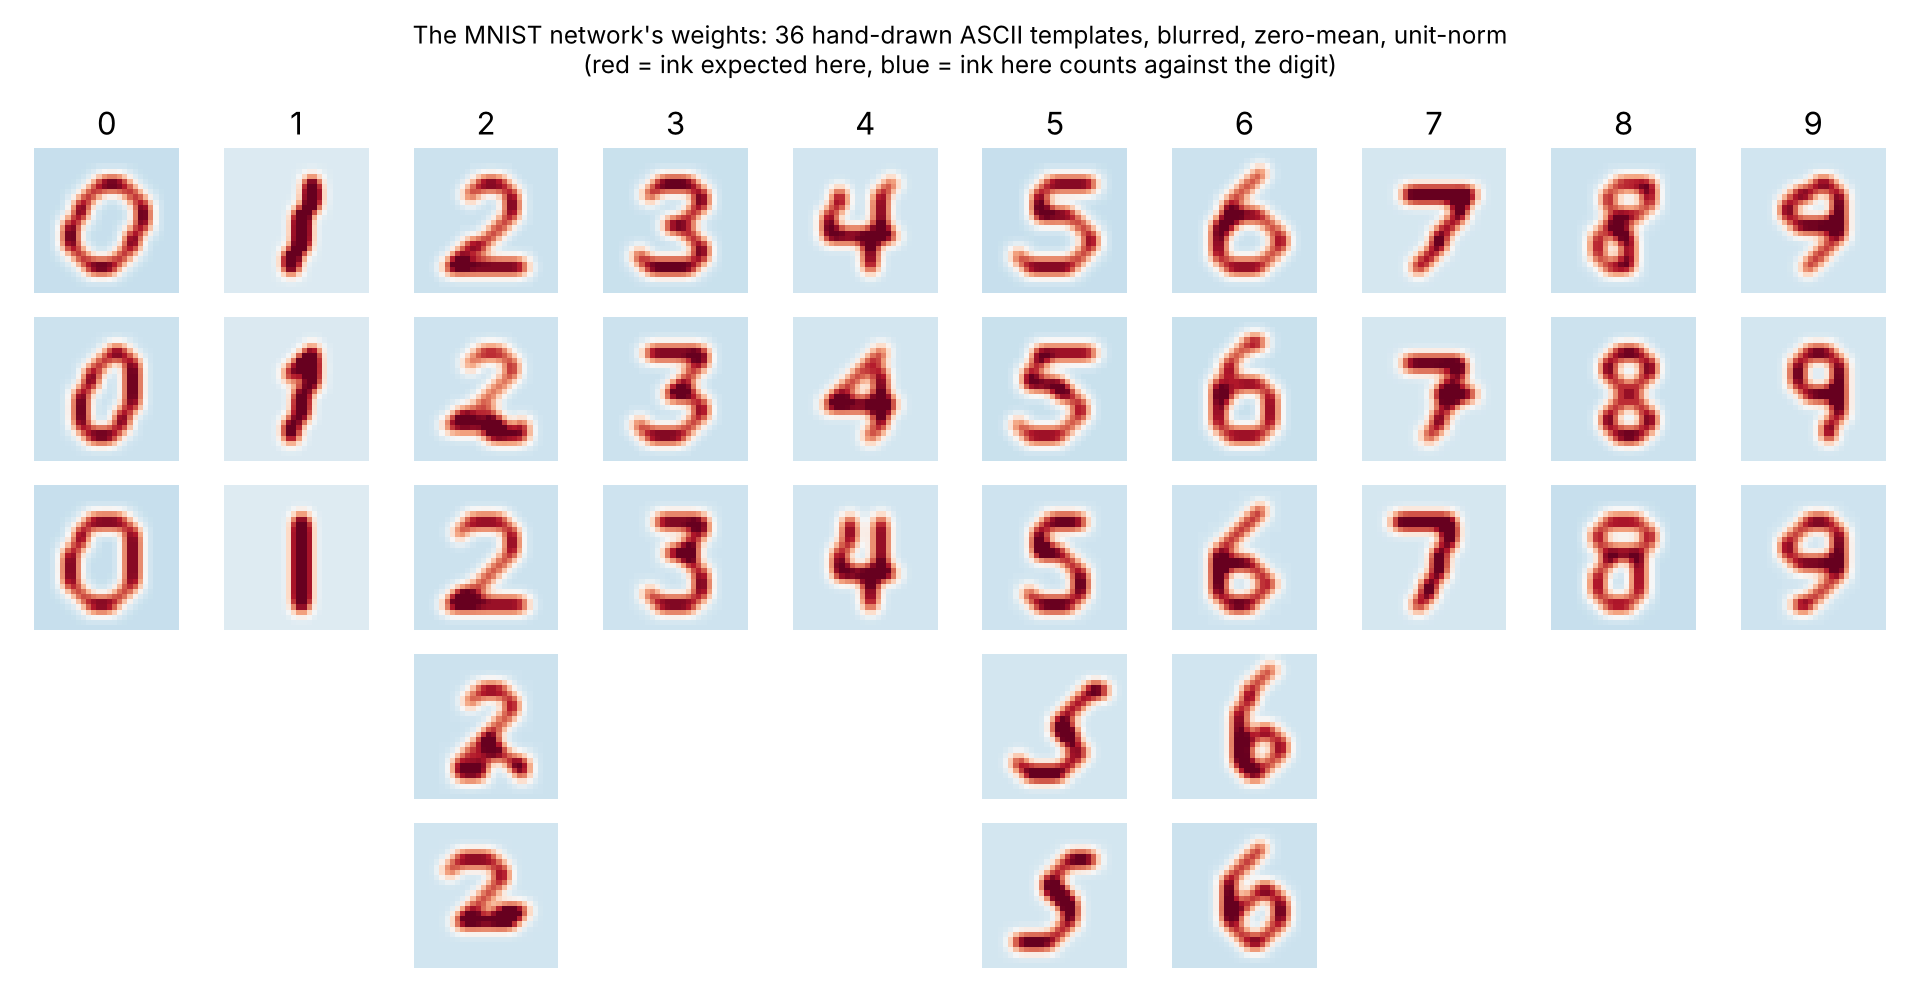
\includegraphics[width=\linewidth]{figures/mnist_templates.png}
\caption{The MNIST network's weights: 36 hand-drawn templates after expansion to
$28\times28$ kernels. Red: ink expected; blue: ink here is evidence against the digit.}
\label{fig:templates}
\end{figure}

\begin{table}[h]\centering
\begin{tabular}{lrrr}\toprule
Weights & Labels seen & Ink pixels / templates & Test acc.\\\midrule
\textbf{Hand-drawn} & 0 & 544 / 28 & \textbf{55.4\%}\\
\textbf{Hand-drawn, revision 1} & 500 (class means viewed) & 553 / 30 & \textbf{74.3\%}\\
\textbf{Hand-drawn, revision 2} & 500 (error images viewed) & 662 / 36 & \textbf{79.4\%}\\
Trained logistic regression & 50 & -- & 61.4\%\\
Trained logistic regression & 100 & -- & 71.5\%\\
Trained MLP (64 hidden) & 100 & -- & 71.8\%\\
Trained logistic regression & 500 & -- & 85.0\%\\
Trained MLP (64 hidden) & 500 & -- & 86.2\%\\
Trained logistic regression & 10{,}000 & -- & 90.9\%\\
Trained MLP (64 hidden) & 10{,}000 & -- & 95.4\%\\
\bottomrule\end{tabular}
\caption{MNIST test accuracy. The best hand-drawn network is worth about 200
labelled images.}
\label{tab:mnist}
\end{table}

\paragraph{Revisions.} The blind drawings were systematically wrong: one grid row
too high, upright rather than right-leaning, too wide. Revision~1 redrew all ten
digits after viewing the class-mean image of 500 labelled training digits next to
the templates ($+19$ points). Revision~2 added two styles each for 2, 5 and 6 (the
weakest classes) after viewing six misclassified training examples of each, widened
the blur from $3\times3$ to $5\times5$ and the shift from $\pm2$ to $\pm3$\,px
($+5$ points).

\paragraph{Why this one loses.} The large confusions are $3\to5$ (197), $4\to9$
(158), $9\to4$ (129) and $5\to8$ (106): pairs that differ in the presence of one
small stroke, which a whole-digit correlation barely registers against the shared
bulk of the shape. A trained linear classifier puts large weight on exactly those few
discriminative pixels; a person drawing a prototype cannot know which pixels those
are without seeing thousands of examples. The features that matter on MNIST are not
nameable, so the design step has nothing to work with. A part-based variant
(hand-drawn stroke detectors feeding a hand-written $10\times64$ linear layer) was
tried and abandoned: writing those 640 numbers was, on inspection, guessing.

\begin{figure}[t]\centering
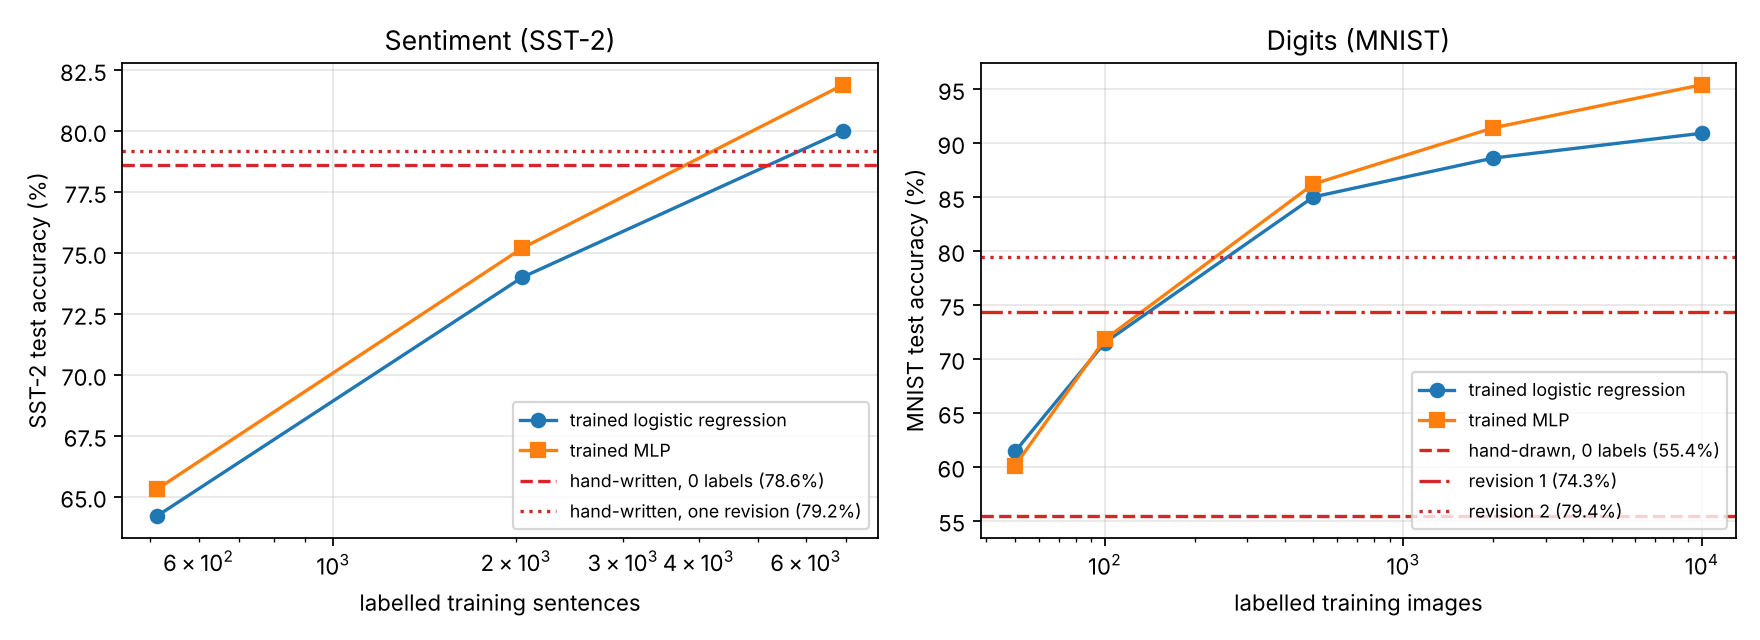
\includegraphics[width=\linewidth]{figures/label_efficiency.png}
\caption{Designed versus trained, per label. Dashed lines: hand-written networks;
curves: the same architectures trained on $2^k$ labels. Sentiment (left) and MNIST
(right) sit at the two ends of the ``nameable features'' axis.}
\label{fig:labels}
\end{figure}

% Experiments: hand-written MNIST classifier. Owner: claude (mnist thread, 2026-11-04).
\subsection{MNIST, second design: a hole finder, sketches and evidence}
\label{sec:mnist-holes}

\paragraph{Task and relation to Section~\ref{sec:mnist}.} The same task, approached by a
second thread independently and under a different protocol. Where the network of
Section~\ref{sec:mnist} was written blind and then revised twice, this one was designed
with the training set in view from the start (see ``How the numbers were set'' below), so
its number is not a blind-write result and is reported separately. Its design differs in
three ways: a recurrent \emph{hole finder} computes the topology that a feed-forward
template cannot, the sketches are drawn per \emph{stroke-orientation channel} rather than
on raw ink, and a layer of named evidence units votes on the confusions that prototypes
leave.

\paragraph{Design.} The design question was ``what does a person look at to tell
digits apart?'', and the network is that answer written as units
(Figure~\ref{fig:holes-pipeline}).

\begin{figure}[t]\centering
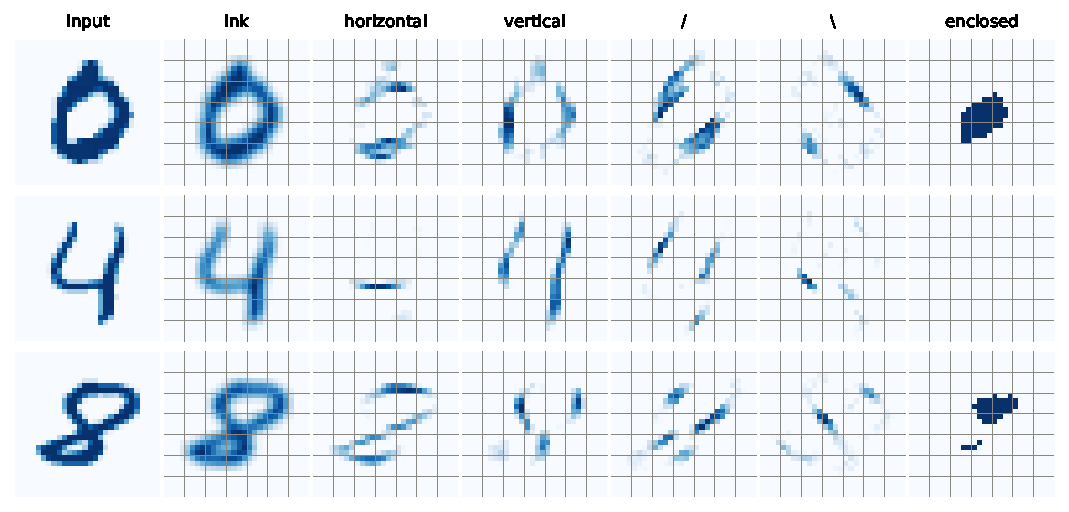
\includegraphics[width=\linewidth]{figures/holes_mnist_pipeline}
\caption{Three test digits through the network: the input, the five hand-drawn
convolution channels, and the output of the recurrent hole finder. The grid is the
$5\times5$ zone pooling. Note the 8 whose lower loop did not close: the single most
common error.}
\label{fig:holes-pipeline}
\end{figure}

\emph{Kernels.} Five $5\times5$ kernels: a $3\times3$ box blur for \emph{ink}, and
oriented-bar detectors for horizontal, vertical, ``/'' and ``\textbackslash'' strokes
($+1$ on the bar, $+1.5$ at the centre, $-0.25$ beside it, divided by 4, bias $-0.15$).
A stroke lights its own orientation and, because of the negative surround, not the
others.

\emph{Hole finder.} Holes---the enclosed background of a 0, 6, 8 or 9---are the strongest
single cue a person uses, and they are topological, which a feed-forward convolution
cannot compute. We compute them with a ReLU recurrence over the image. Let $b$ be the
background (ink below $0.3$). Seed $r_0$ with the border of $b$ and iterate
\[
r_{t+1} = \mathrm{relu}\big(\min(1,\textstyle\sum_{3\times3} r_t) + b - 1\big),
\]
so a background pixel becomes \emph{reached} as soon as it touches a reached pixel.
After 56 steps everything reachable from the border has been reached and $b-r$ is the
enclosed background. This is the same construction as the run-length counters of
Section~\ref{sec:text-quality}---a ReLU recurrence with identity self-connection---applied
over an image instead of a string.

\emph{Zone pooling.} All six maps (five conv channels and the hole map) are averaged over
a $5\times5$ grid of $4\times4$-pixel zones covering the central $20\times20$ box in which
MNIST digits sit: 150 zone features, plus seven globals (ink, hole area, hole area in
the top and bottom halves, width, height, left--right ink balance).

\emph{Sketches.} For each channel, each digit is drawn by hand on the $5\times5$ grid as
ASCII art (Figure~\ref{fig:holes-sketches}): \texttt{\#} strong, \texttt{+} some,
\texttt{.} little, \texttt{-} must be empty. The 60 sketches \emph{are} the weights of 60
units: a sketch $W$ gives the unit $W\cdot x-\tfrac12\|W\|^2$, which up to a constant is
minus the squared distance to the prototype, so the readout asks ``which hand-drawn
digit is this closest to'', channel by channel (channel weights: ink 1, strokes 2,
``\textbackslash'' 1, hole 4). The sketches were drawn after looking at what MNIST digits
look like at this resolution---slanted 1s, 4s with a stem to the right, 7s whose roof
sits on the second row---the way a person who has seen handwriting draws a digit, and
are deliberately coarse.

\begin{figure}[t]\centering
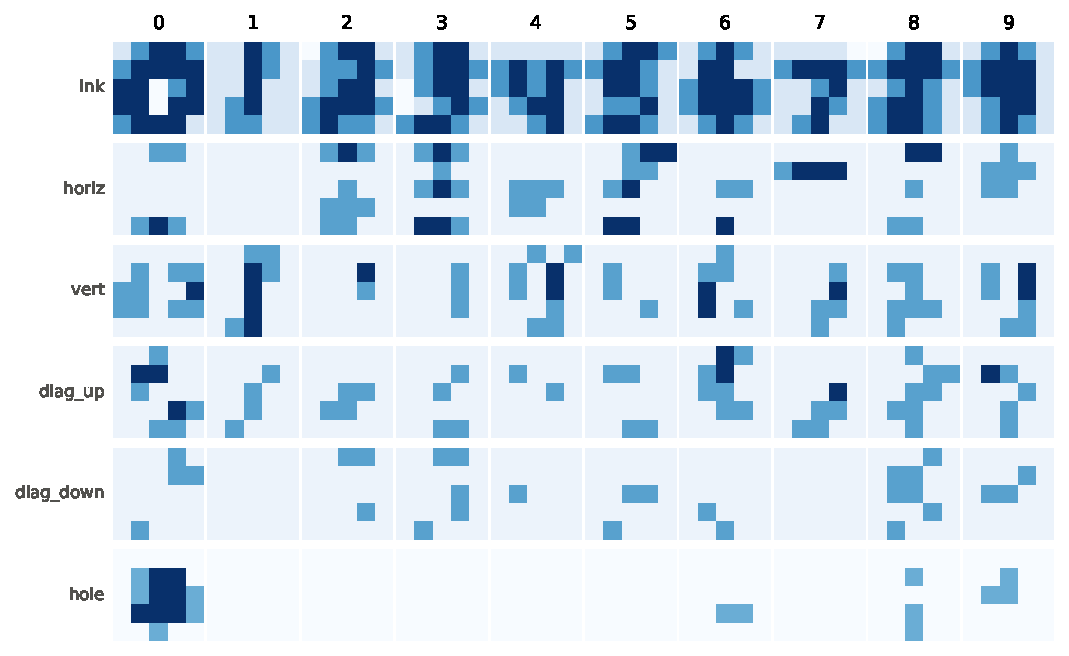
\includegraphics[width=\linewidth]{figures/holes_mnist_sketches}
\caption{The sixty hand-drawn sketches, one per digit and channel. These are the
prototype weights.}
\label{fig:holes-sketches}
\end{figure}

\emph{Evidence units.} Sketches alone reach about 80\,\%. The remaining confusions are
topological and shape facts that distance to a prototype does not capture, so 29 named
evidence units vote for and against digits, each a capped detector
$\min(\mathrm{relu}(w\cdot f+b),1)$ over a few zone features (the construction of
Section~\ref{sec:method-capped}): \texttt{hole:none} (votes for 1 3 4 5 7, against 0 8
9), \texttt{hole:big} (0), \texttt{hole:top\_only} (9), \texttt{hole:bottom\_only} (6),
\texttt{hole:top\_and\_bottom} (8), \texttt{narrow} (1), \texttt{four:open\_top} (two posts
and an empty top centre), \texttt{seven:roof}, \texttt{two:foot}, \texttt{three:bumps},
\texttt{five:corner}, \texttt{six:left\_sweep}, \texttt{nine:stem}, \texttt{zero:ring},
\texttt{eight:waist}, \texttt{bottom\_bar} (0 2 3 5 6 8 have one; 1 4 7 9 do not),
\texttt{roof\_row1} (a 7, never a 4), \texttt{top\_centre\_filled} (against 4),
\texttt{has\_horizontals} and \texttt{has\_backslashes} (against 1), and a few more.
In total $|\theta|=21{,}772$ and $\|\theta\|_0=2{,}411$.

\paragraph{How the numbers were set.} The kernels, the hole finder, the sketches and the
unit definitions were written from how digits look. Thresholds were placed by reading
class-conditional means of the zone features on the first 5{,}000 \emph{training} images
and putting the knee between a digit and its neighbours (``a 4's top-centre ink is 0.6, a
9's is 1.8, so threshold at 1.0''). Vote weights were then adjusted by hand over about a
dozen rounds of looking at the confusion matrix on those same 5{,}000 images and asking
which unit was to blame for each confusion. No gradient, optimiser or search over weights
was used. A held-out training slice (images 5{,}000--10{,}000) gives 82.8\,\%, so the hand
tuning did not overfit; the test set was scored once, at the end.

\paragraph{Results.} On the 10{,}000 MNIST test images the network is \textbf{83.3\,\%
accurate} (Figure~\ref{fig:holes-confusion}), at $0.9$\,ms per image in NumPy. The
majority class gives 11.4\,\%. A \emph{trained} nearest-class-mean classifier on the raw
784 pixels (ten prototypes fit on 20{,}000 training images) gives 81.6\,\%, so ten digits
drawn by hand on a $5\times5$ grid, plus the hole finder and a page of evidence, do
slightly better than ten prototypes fit to data at full resolution. A trained
convolutional network reaches over 99\,\%. Per-class accuracy ranges from 95\,\% (1) and
91\,\% (2, 3) down to 77\,\% (5, 9) and 65\,\% (8).

\begin{figure}[t]\centering
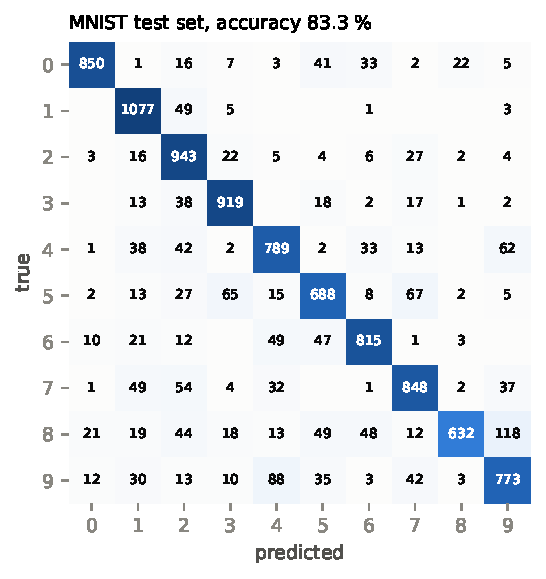
\includegraphics[width=0.5\linewidth]{figures/holes_mnist_confusion}
\caption{Confusion matrix on the 10{,}000 MNIST test images (rows normalised for colour).}
\label{fig:holes-confusion}
\end{figure}

\paragraph{Where it fails, by construction.} The errors are the ones a $5\times5$ sketch
would be expected to make, and the hole finder explains most of them: 8$\to$9 (118 cases)
when the lower loop did not close, 9$\to$4 (88) when the upper loop did not close,
4$\to$9 (62) when a 4 is written with a closed top; and the shape pairs 5$\to$7 (67) and
5$\leftrightarrow$3 (65), where a 5 with a short roof is a 3 with a corner. The unit
firing rates on the test set confirm the picture: \texttt{hole:none} fires on 99\,\% of 1s,
3s, 5s and 7s but also on 26\,\% of 9s and 37\,\% of 6s, which is where the accuracy
goes. A $5\times5$ sketch cannot say ``the loop must close'', and the hole finder cannot
close a loop the writer left open; a trained network learns the fine stroke-topology
statistics that fill that gap, and that is exactly the part of the task a designer
cannot write down.


\section{Discussion and limits}
% Discussion seed from the sentiment/MNIST thread; the paper thread may restructure.
\subsection{When does writing beat training?}
The three networks line up on one axis: how \emph{nameable} the discriminative
features are (Table~\ref{tab:when}). Where an expert could write the rules as a list
---this word is positive, negation reaches three words, mojibake looks like
\texttt{\~A\textparagraph}---the rules map one-to-one onto units and the designed
network is competitive with thousands of labels. Where the features are statistical
regularities in pixel space that nobody can enumerate, a few hundred labels beat the
best drawings anyone can make. Lauritzen's legal-citation task \cite{lauritzen2026}
sits at the far nameable end (reporter names, volume and page formats), which is why
designed weights beat 8{,}192 labels there.

\begin{table}[h]\centering\small
\begin{tabular}{lp{3.2cm}p{3.4cm}p{3.2cm}}\toprule
 & Sentiment & Text quality & Digits\\\midrule
Input unit & word & character attribute & pixel\\
Nameable features? & yes: lexicon, negation, contrast & yes: markup, repeats, mojibake, lengths & no\\
Designed vs trained & wins up to $\sim$3{,}000 labels & AUC 0.86--0.95, no labels & loses beyond $\sim$200 labels\\
Ceiling & syntax, irony & grammar & fine stroke differences\\
\bottomrule\end{tabular}
\caption{Where hand-written weights are competitive.}\label{tab:when}
\end{table}

\subsection{The revision step is where the labels go}
A revision after inspecting 500 labelled examples is not zero-label learning; it is
hypothesis-driven learning with very few degrees of freedom. The right comparison for a
revised designed network is a trained one at the same label count, which is why every
table lists labels seen. On MNIST the revised network (500 seen, 79.4\%) loses to a
trained one on 500 labels (85--86\%); on SST-2 the revised network (872 seen, 79.2\%)
beats a trained one on 2{,}048.

\subsection{A capability measurement}
``Can model $M$ write the weights of a working classifier for task $T$?'' has a numeric
answer; it differs across tasks in an interpretable way; and it will presumably rise
across model generations. A model that writes a 79\% MNIST classifier from an
ASCII-art prior and a 79\% SST-2 classifier from its own lexicon is telling us something
about what it knows that a multiple-choice benchmark does not.

\subsection{Things that went wrong}
Dual-role words (\emph{never} as negator and as negative) need an explicit decision.
The blind MNIST drawings were one row too high; a single \emph{unlabelled} look at the
input distribution would have prevented this and a future protocol should allow it.
``Painfully funny'' was scored as \emph{painful}+\emph{funny}; intensifier readings of
negative adverbs are real in review English. A document-length penalty appropriate for
pretraining filtering dominates single sentences. And when a weight cannot be
justified in a sentence---as in the abandoned part-based MNIST net---that is the signal
to stop.

% Discussion paragraphs from the mnist_holes / 33-language thread; additive to discussion.tex.
\subsection{What reasoning buys, and where it runs out}
\paragraph{What reasoning buys.} The text-quality and hole-finder networks were written in a few hours of
conversation and have no training cost, and both land at the level of the classical
hand-engineered baselines for their tasks: the text gate reproduces most of a production
filtering pipeline's decisions across 33 languages, and the second digit classifier beats a trained prototype classifier. Both are entirely legible: every score decomposes into named
contributions, which is what a data engineer wants from a filter (``why was this document
dropped?'') and what makes the error analyses above possible without any probing.

\paragraph{Where reasoning runs out.} The failures are informative. The text network
cannot see grammar, because that needs a representation of words and their order, which
no amount of character-level reasoning produces; and the 33-language ablation shows that
several detectors that are easy to justify contribute nothing measurable. The digit
network's ceiling is set by the resolution of what a person can specify: a $5\times5$
sketch cannot say ``the loop must close'', and the hole finder cannot close a loop the
writer left open. A trained network learns the fine stroke-topology statistics that fill
that gap, and that is exactly the part of the task a designer cannot write down.

\paragraph{Fine-tuning from a designed initialisation.} Because these are ordinary networks
with PyTorch exports (\texttt{to\_torch()}, checked against NumPy in the tests), the
obvious next experiment is to use them as initialisations: does a network that starts
from named, correct detectors train faster, need fewer labels, or stay legible? The
repository deliberately does not run that experiment yet, so that the reported numbers
are those of the hand-written weights alone.

\paragraph{On process.} The weights were written by a language model in conversation with
the first author, who set the tasks, the rule (reason and check, never fit) and the
standard of evidence. We think this is worth stating because it bears on what the result
means: the design knowledge in these networks is the kind that can be articulated---what
mojibake looks like, where a 4 is empty---and a system that can articulate it can also
write it into weights. The repository documents the process, including the development
log of Section~\ref{sec:tq-devlog} and the iteration on training-set confusion matrices
for MNIST, so that the line between ``reasoned'' and ``fit'' is visible to the reader.


% Seeds kept from the first draft:
% - Grammar at chance: the input carries no morphology; this is a representational limit,
%   not a tuning one. Designed nets are bounded by what the author can articulate in the features.
% - Fluent machine-translated spam scores 95+: surface shape is all the network sees.
% - What training adds: initialise the same architecture from the designed weights and
%   fine-tune on FineWeb-2 labels; report accuracy vs number of labels (the Lauritzen table).
% - Designed nets as specifications: a threshold change is a one-line edit with a known effect;
%   tests pin behaviour; the model is reviewable like code.
% - Cost: ~7 ms/doc numpy, no GPU; ~1000x cheaper than a 0.3B judge.

\section{Conclusion}
Two ordinary networks, no training, every weight decided: a text-quality gate that agrees
with FineWeb-2's filters at AUC 0.907 across 33 languages with 627 non-zero weights, and an
MNIST classifier at 83.3\,\% built from hand-drawn kernels, a hole-finding recurrence and
ten digits sketched on a $5\times5$ grid. Reasoning gets a network to the level of the
classical hand-engineered baselines, makes every decision legible, and stops exactly where
the task knowledge stops being articulable. That boundary is itself a result, and the
networks are released as initialisations for anyone who wants to measure what training
adds on top of design.

\bibliographystyle{plain}
\bibliography{refs}

\end{document}
